\section{Experiments}\label{sec:expts}

\begin{table}[h]
\centering
\small
 \setlength{\tabcolsep}{4pt}
\begin{tabular}{p{1.8cm} l l l@{\hskip 0.4cm} l@{\hskip 0.5cm} l l@{\hskip 0.5cm} l l }
\toprule
Dataset & \#folds/ & \#users & \#items & train & \multicolumn{2}{l}{test} & \multicolumn{2}{l}{\#features} \\
              & samples &              &               & \#pairs  & \#pairs & \#scores          & items & users \\
\midrule
Simulation a & 25 & 25 & 100 & 900 & 0 & 100 & 2 & 2 \\
Simulation b & 25 & 25 & 100 & 900 & 0 & 100 & 2 & 2\\
Simulation c & 25 & 25 & 100 & 36--2304 & 0 & 100 & 2 & 2\\
\midrule
Sushi A-small & 25 & 100 & 10 & 500 & 2500 & 1000 & 18 & 123 \\
Sushi A & 25 & 100 & 10 & 2000 & 2500 & 1000 & 18 & 123 \\
Sushi B & 25 & 5000 & 100 & 50000 & 5000 & 500000 &  18 & 123 \\
\midrule
UKPConvArg-CrowdSample & 32 & 1442 & 1052 & 16398 & 529 & 33 & 32310 & 0
\\ \bottomrule
\end{tabular}
\caption{Summary of datasets showing counts per subsample. 
For simulations, we generate the subsamples of data independently, 
for Sushi we select subsamples independently from the dataset.  
Values for UKPConvArgCrowdSample are means per fold, 
where the test data in each fold corresponds to a single topic and stance. 
Numbers of features are given after categorical labels have been converted to one-hot encoding, counting
each category as a separate feature.
}
\label{tab:datasets}
\end{table}
Our experiments test the key aspects of \emph{crowdGPPL}: 
 modelling personal preferences from pairwise labels;
 predicting consensus utilities from noisy crowdsourced preferences
  in a subjective task; 
 and the scalability of our proposed SVI method.
In Section \ref{sec:exp_synth}, we use simulated data to test the robustness of crowdGPPL
to noise and unknown numbers of latent components.
Section \ref{sec:sushi}, 
compares different configurations of the model
against alternative approaches
using the \emph{Sushi} datasets\footnote{\url{http://www.kamishima.net/sushi/}}~\citep{kamishima2003nantonac}.
Section \ref{sec:exp_scale} evaluates 
the ability of crowdGPPL to predict both personal and consensus utilities 
in a high-dimensional
natural language processing (NLP) task
with sparse, noisy crowdsourced preferences
(\emph{UKPConvArgCrowdSample}\footnote{\url{https://github.com/ukplab/tacl2018-preference-convincing}}, ~\citet{simpson2018finding}).
Using the same dataset, Section \ref{sec:exp_scale} analyses
the scalability of our SVI approach. 
Finally, Section \ref{sec:components} evaluates whether crowdGPPL ignores redundant
components when the number of components, $C$,
is larger than necessary.
The datasets are summarised in Table \ref{tab:datasets}.

\subsection{Method Comparison}

% Ranking-SVM baseline -- only easy to compare in the single user case. My GPPL paper perhaps needs
% this adding in any follow up works.

% Houlsby tests: with/without user features (without is better with few users). + a hierarchical 
% model, BI (multi task preference learning, Birlitiu et al), and the GPPL-joint model. None of 
% these are done at scale, which we can do with our inference method --> *this is a new claim i.e. 
% new empirical results*. They also test a per-user model.

As baselines, we compare crowdGPPL against 
\emph{GPPL},
which we train on all users' preference labels to learn a single utility function,
%and a Gaussian process over the joint feature space of users and items 
%(\emph{joint-GPPL}), as proposed by \citet{guo2010gaussian}.
and \emph{GPPL-per-user},
in which a separate GPPL instance is learned for each user with no collaborative
learning.

The \emph{collaborative Gaussian process} (\emph{collabGP}, ~\citet{houlsby2012collaborative}), 
is a similar model that, like crowdGPPL,
 assumes Gaussian processes over latent user and item components,
 but does not learn a consensus or the scales of the components to 
 identify active and unneeded components.
 The inference method uses an inducing point method, \emph{GFITC}, 
 to obtain linear time complexity. It
 maintains a set of parameters for each pairwise label and
 for each user, so unlike our SVI scheme, its memory complexity 
grows with the number of pairs in the dataset
($\mathcal{O}(M_{\mathrm{items}}P + M_{\mathrm{users}}U)$
in contrast to 
$\mathcal{O}(C M_{\mathrm{items}} P_i + C M_{\mathrm{users}} P_i$).
We therefore treat the performance of collabGP as a target for the smaller crowdGPPL model,
which does not retain parameters specific to each user or item in the dataset.

\emph{CrowdBT}~\citep{chen2013pairwise}
has been shown to be an effective method for learning from crowdsourced preferences.
CrowdBT learns a model of each worker's accuracy and infers consensus utilities, 
therefore assuming that the differences between workers' labels are 
due to random errors rather than subjective preferences.
Since crowdBT does not account for the item features,
it cannot predict utilities for items that were not part of the training set
and is hence purely an aggregation method.
However, the aggregated utilities produced by crowdBT can be treated as training labels
for regression. Here, we use the posterior mean utilities from crowdBT 
as target values for training a Gaussian process regressor,
and set the observation noise variance of the GP equal to the posterior variance
of the utilities estimated by crowdBT. 
This pipeline method, \emph{crowdBT--GP}, 
allows us to test whether it is sufficient to treat annotator differences as noise,
or whether it is beneficial to use the
crowdGPPL approach of modelling individual preferences of annotators.


\subsection{Simulated Noisy Data}\label{sec:exp_synth}

First, we compare crowdGPPL to the baselines to see if it is able to model individual preferences
with varying amounts of labelling noise. 
We set $C=20$
and for all models, we set all the Gamma hyperparameters to 
$\alpha_0 = 1$, $\beta_0 = 100$,
and use Mat\'ern 3/2 kernels with length-scales chosen by a median heuristic:
\begin{flalign}
 l_{d,MH} = \sqrt{D} \times \mathrm{median}( \{ ||x_{i,d} - x_{j,d}||, 
 \forall i=1,..,N, \forall j=1,...,N\} ),
\end{flalign}
where $D$ is the dimension of the input feature vectors.
The median heuristic is a computationally frugal heuristic for choosing the length-scales,
which effectively normalizes the features and has been extensively used
in various kernel methods (e.g., ~\citet{bors1996median,gretton2012optimal}).
The kernels for each dimension are multiplied together, so 
multiplying the length-scales by $\sqrt{D}$ prevents the average covariance between items or users 
from shrinking as the number of features grows.
% This heuristic has been shown to work reasonably well for the task of 
% comparing distributions, but has %is a simple heursitic with
%  no guarantees of optimality. 
The SVI hyperparameters were set to 
 $\rho=0.9$, $P_i=1000$ and $\epsilon=1$.
 \citet{hoffman2013stochastic} found that higher values of 
 $\rho$ gave better final results but slightly slower convergence, recommending
 $0.9$ as a good balance, and did not find any effect from changing $\epsilon=1$. 
 They also found that increasing batch size $P_i$ improves performance, 
 however this is likely to be constrained in practice by the size of the batch that the 
 computer can process.
 While $\rho=0.9,\epsilon=1$ are recommended as sensible defaults, 
 these hyperparameters may need some light tuning to a specific dataset,
 e.g. using grid search to maximise the lower bound of the log marginal likelihood, $\mathcal{L}$.
 
First, to test prediction of the consensus,
we generate data by creating a $20\times 20$ grid of points, choosing $400$ pairs of these points at random, and splitting them into  50\% training and test sets.
For each point, we generate pairwise labels by drawing from crowdGPPL
with $20$ users, $5$ latent components, and 
$s^{(v)}_c = s^{(w)}_c = 0.001$, for all components.
We vary the precision of the consensus function, $s^{(t)}$, 
to control the noise in the consensus function. 
The complete experiment was repeated $25$ times, including generating new data 
for each value of $s^{(t)}$.
Figure \ref{fig:simB} shows that crowdGPPL is better able to recover the 
consensus ranking than the other methods, even when noise levels are high. 
GPPL's predictions may be worsened by biased users whose preferences deviate
consistently from the consensus. 
For GPPL-per-user, the consensus is estimated by taking
the mean of all users' predicted utilities, 
GPPL-per-user relies on separate instances of GPPL
and estimates the consensus by taking the mean of all users' predicted utilities, 
so does not benefit from sharing information between users when training.

The second simulation modifies the previous setup by fixing $s^{(t)} = 10$ and varying $s^{(v)}_c,\forall c$
to evaluate the methods'
ability to recover the personal preferences of simulated users.
Results in Figure \ref{fig:simC} show that crowdGPPL is able to make better 
predictions when noise is below $0.3$ but its benefit disappears when 
the noise level increases further. 

\begin{figure}[t]
%\subfloat[Inferring preferences for a single user]{
%\label{fig:simA}
%\includegraphics[width=.35\columnwidth]{../../results/synth_3/single_user/tau_test}
%}
\subfloat[Consensus]{
\label{fig:simB}
\includegraphics[width=.322\columnwidth,clip=true,trim=11 0 13 0]{tau_test}
}
\subfloat[Personal preferences]{
\label{fig:simC}
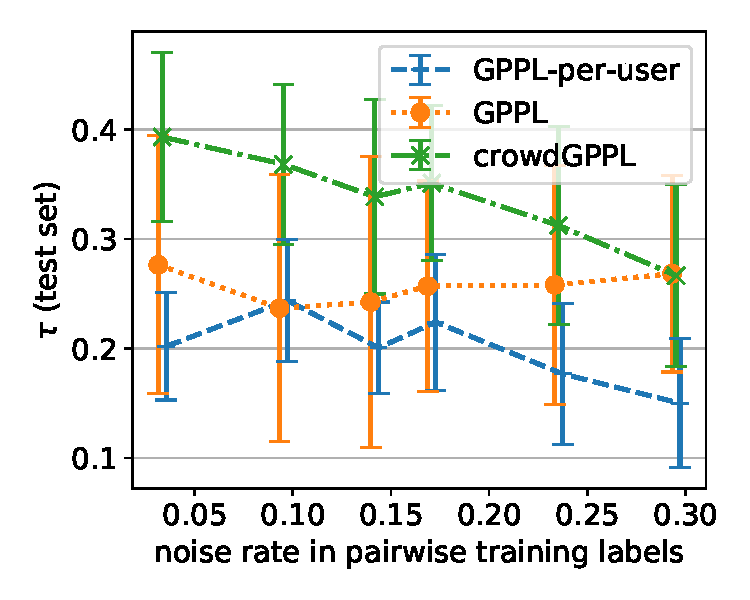
\includegraphics[width=.316\columnwidth,clip=true,trim=20 0 13 0]{tau_test_personal}
}
\subfloat[Latent factors]{
\label{fig:simD}
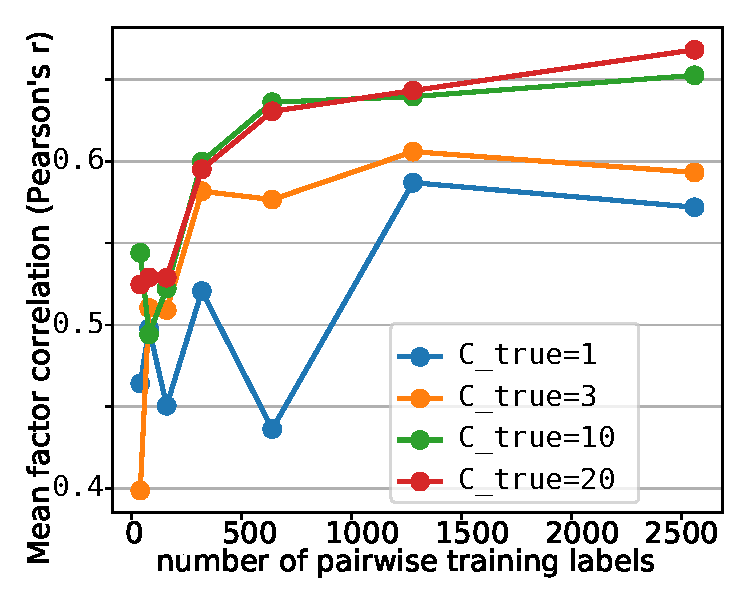
\includegraphics[width=.325\columnwidth,clip=true,trim=11 0 12 0]{num_pairs_r}
}
\caption{Simulations: Rank correlation between true and inferred preference values for different inference tasks.  (a) \& (b) varying level of noise in pairwise training labels, (c) varying number of pairwise training labels. 
}
\end{figure}
\todo{
 Page 14, Figure 1: include error bars, especially in sub-figure (c).
}
%In the final simulation, %we evaluate the effect of the quantity of training data 
%with different numbers of latent factors in the generating model.
We hypothesize that learning a model with a larger number of latent components
requires more training data.
%scenario that would require more training data. 
In the third simulation, we generate data using the same setup as before, but fix $s^{(v)}=0.2,\forall c$ and $s^{(t)}=1$
and vary the number of pairwise training labels 
and the number of true components through
$C_{true} \in \{ 1, 3, 10, 20\}$.
To evaluate the correlation between inferred and true user components, 
%we match inferred factors to true factors, 
we compute Pearson correlations between each
true component and each inferred component, then repeatedly select pairs of components with the highest correlations
 until every true component is matched to an inferred component. 
In Figure \ref{fig:simD} we plot the mean of the correlations between matched pairs of components.
For all values of $C_{true}$, increasing the
number of training labels beyond $1000$ leads to only minor increases in correlation at best. 
Performance is highest when $C_{true} = 20$,
possibly because the predictive model has $C = 25$
and hence is a closer match to the generating model.
However, for all values of $C_{true}$, performance with $>500$ labels remains above 0.5,
 showing the model is reasonably robust
to mismatches between $C$ and $C_{true}$.
% Does this pose a question: does the mismatch affect the performance? If the correlations
% decrease, it may mean that the model is decomposing a factor into a sum of multiple factors,
% or it may just be unable to learn it. This would need a new experiment: for 700 training pairs,
% how does the accuracy of personalised predictions vary with the number of latent factors?
% I think this needs us to vary C and keep C_true=3, otherwise we don't know whether the 
% performance differences are due to the mismatched no. factors or due to different underlying dataset, i.e. we need to keep the data the same to compare!


\subsection{Sushi Preferences}\label{sec:sushi}

%TODO sushi-A small needs describing or cutting out.
We use sushi preference data (shown in Table \ref{tab:datasets}),
to compare GPPL and crowdGPPL with different sets of features
against the previous benchmark method, \emph{collaborative GP (collabGP)} \citep{houlsby2012collaborative}.
Collaborative GP uses a simpler model than crowdGPPL, with no consensus function, and no learning of the 
output scales of the utility functions, which makes it more important to select the correct number of factors in advance.
It also uses an inference scheme based on expectation propagation (EP)
 and variational Bayes, which has a couple of important
  practical drawbacks:
  firstly, it does not infer the utilities, but learns pairwise labels directly, so its predictions cannot 
  directly be used to
  rank or rate large sets of items; 
  secondly, the number of parameters in the model is proportional to the dataset size, 
  as it represents every combination of
  (user, item-pair) with a separate set of parameters, rather than working with inducing points,
  which may prevent the use of the model with large datasets due to memory constraints.
However, as the EP approach of collabGP has been consistently shown to perform well for non-Gaussian likelihoods\citep{?},
we consider its performance as a target for our SVI approach for crowdGPPL.

The sushi datasets contain, for each user, a gold standard preference ranking 
of $10$ types of sushi,
from which we generate gold-standard pairwise labels. 
%These labels can be considered noise-free, since
%they are derived directly from the gold standard ranking.  
To test performance with very few training pairs, we obtain \emph{Sushi-A-small}
by selecting $100$ users at random from the complete \emph{Sushi-A} dataset,
then selecting $5$ pairs for training and $25$ for testing per user.
For \emph{Sushi-A}, we select a subset of $100$ users at random from the complete dataset, then 
split the data into training and test sets by randomly
selecting $20$ pairs for each user for training and $25$ for testing. 
For \emph{Sushi-B}, we use all $5000$ workers, and subsample $10$ training pairs and $1$ test pair per user.
%These subsampling steps are repeated $25$ times.
Beside GPPL, crowdGPPL and GPPL-per-user, we 
% but this could not be applied to larger datasets as the 
%computation costs were too high.
introduce four further baselines: 
\emph{crowdGPPL$\mathbf{\backslash \bs u}$}, which ignores the user features;
 \emph{crowdGPPL$\mathbf{\backslash \bs u \backslash \bs x}$}, which ignores both user and item features;
 \emph{crowdGPPL$\mathbf{\backslash \bs u \backslash \bs t}$}, which 
excludes the consensus function $\bs t$ from the model as well as the user
features;
and  \emph{crowdGPPL$\backslash$induc}, which uses all features but does 
not use inducing points for a sparse approximation.
For $\backslash\bs u$ methods, the user covariance matrix, $\bs K_w$, in the crowdGPPL model is replaced by the identity matrix, and for crowdGPPL$\mathbf{\backslash \bs u \backslash \bs x}$, the item covariance matrices, $\bs K_v$ and $\bs K_t$ are also replaced by the identity matrix.
%We evaluate the quality of pairwise predictions using classification accuracy and cross entropy 
%error (also known as log loss) to gauge the quality of the probabilities that each method outputs.
%We also evaluate each method's inferred personal preference values
%against the gold standard rankings by computing Kendall's $\tau$ rank correlation
%coefficient between the negative rank and the inferred preference function values,
%for all the items contained in each subsampled user's ranking.
We set hyperparameters $C=20$ without optimization,
$\alpha_0=1, \beta_0=100$ using a grid search over values 
$10^{\{-1,...,3\}}$ on withheld user data from the \emph{Sushi-A} dataset,
\todo{clarify the parameters for sushi and for conv}
$\epsilon=5$, $P_i=200$ for \emph{Sushi-A} and $P_i=2000$ for \emph{Sushi-B}. All other hyperparameters are the same 
as for Section \ref{sec:exp_synth}.
The complete process of subsampling, training and testing, was repeated $25$ times
for each dataset.

% Houlsby results: for comparison against a different inference technique on small data, include
% the test error results from their paper.
% Guo results: not directly comparable. We will rerun a similar approach but with our inference method.
% Khan results: for a different model that separates the latent features from the item/user features.
% Abbasnejad results (community-based preference learning): sushi data with 10 items; 60/40 train/test split of each user's preference pairs. This means the result is based on 27 pairs training.
% don't worry about this though, it doesn't seem to work very well in their results.

% Number of users affects value of including user features.
% Plot results on increasing dataset size.

% [10] T. Kamishima. Nantonac collaborative filtering:
% Recommendation based on order responses. In
% ACM SIGKDD 9th Int. Conf. Knowledge Discov-
% ery and Data Mining, 2003.

% Run 25 repeats of random train/test splits with:
% Exclude these two as we focus on bigger datasets in this paper. Cutting these creates the space 
% for including three metrics.
% Downside: cannot test whether increasing no. users imroves performance through better collaborative learning. 
% 
% 100 (a la Houlsby 20 pairs per user), 
% 200 (a la Khan, 3 training, 1 test, P=600, P_test=200), 
% For small datasets, we may want to test on the argumentation data so we can assess the crowd
% consensus results with small data. That dataset is more interesting here because lots of items,
% small data is a new scenario.
% % % % [a] 1000 (a la Houlsby 15 training, 5 test pairs per user, $P=15000,P_{test}=5000$), Sushi-A (10 items), 
% % % % and [b] 5000 users (a la Khan, 10 training, 1 test pairs per user, $P=50000, P_{test}=5000$), \emph{Sushi-B} (100 items).
% % % % Evaluate on parwise labelling error, pairwise label logloss, spearman rank correlation,
% % % % and runtime.
% could use normalized mean loss from guo, but not sure where the utilities come from -- ranking?

% 25 random train/test splits on all 5000 users with varying no. (1, 5, 10, 20, 40) pairs per user.

% Can put in the Houlsby (100/1000 users, 20 pairs each, labelling error) and Khan (200 users, 3 pairs each, logloss) results.
% Khan also provide code, so could be rerun to get classification error.

\begin{table}
 \centering
 \small
 \setlength{\tabcolsep}{4pt}
 \begin{tabular}{l l l l@{\hskip 0.5cm} l l l@{\hskip 0.5cm} l l l}
\toprule
& \multicolumn{3}{c}{\textbf{Sushi-A-small}} & \multicolumn{3}{c}{\textbf{Sushi-A}} & \multicolumn{3}{c}{\textbf{Sushi-B}} \\ 
Method & Acc & CEE & $\tau$ & Acc & CEE & $\tau$ & Acc & CEE & $\tau$ \\
\midrule
%\multicolumn{13}{|l|}{\textit{crowdGPPL}} \\
crowdGPPL & \textbf{.71} & \textbf{.56} & .48 %& 38%
& .84 & .33 & .79 %& 21
& .76 & .58 & . 53 %& .76 & .55 & .45  %& 4724 \\
 \\
crowdGPPL $\backslash $inducing & .70 & .60 & .45 %& 51 %(14.81) %& .63 (.02) & .68 (.00) & .24 (.03)
% new results 02.04
& .84 & .34 & .78 %& 39
& - & - & - 
\\
crowdGPPL $\backslash u$ & .70 & .58 & .46 &  %9  &%(24.62) %& .65 (.02) & .64 (.03) & .29 (.03)
% new results 02.04:
\textbf{.85} & \textbf{.31} & \textbf{.80} %& 21
& \textbf{.78} & .52 & .57 %& 3788 
\\
%crowdGPPL $\backslash u, C=50$ & .70 & .58 & .46 & .84 & .32 & .80 & 
%\\
crowdGPPL $\backslash u \backslash x$ & \textbf{.71} & .57 & \textbf{.49} & % 5 & %(3.74) %& .65 (.02) & .63 (.02) & .29 (.03)
%new results 02.04: 
\textbf{.85} & .33 & .80 % & 14
& .77 & .50 & .58 % & 3363
\\
crowdGPPL $\backslash u,\backslash t$ % this is also FITC to emulate Houlsby -- mention it in the text, not here
& .68 & .60 & .43 % & 291 %(48.62) %& .50 (.00) & .69 (.00) & nan (nan)
& .84 & .33 & .80 % & 230
& .76 & .50 & .58 % & 12513
\\ 
\midrule 
GPPL & .65 & .62 & .31 %& \textbf{2} %(.26) %& .65 (.02) & .63 (.02) & .30 (.03)
& .65 & .62 & .31 % & \textbf{2}
& .65 & .62 & .31 % & \textbf{51}
\\
GPPL-per-user & .67 & .64 & .42 % & 183 %(1.12) %& .50 (.00) & .69 (.00) & nan (nan)
& .83 & .40 & .79 % & 44
& .75 & .60 & \textbf{.60} % & 3172 %(.44)
\\
collabGP & .69 & .58 & n/a %& \textbf{2}* 
& .83 & .35 & n/a %& 6* 
& .76 & \textbf{.49} & n/a % & 1283* \\
%\citet{houlsby2012collaborative} CPU & & & & & .83 \\ 
%\citet{khan2014scalable} & &&& & & & & & .69 & &
%\\ \hline
\\
collabGP$\backslash u$ & .69 & .59 & n/a & .84 & .33 & n/a & .76 & .50 & n/a
\\
GPVU & .70 & .67 & .43 & .72 & .67 & .42 & .73 & .59 & .52
%collabGP$\backslash u, C=50$ & .70 & .58 & n/a & .85 & .33 & n/a & \\
\\ \bottomrule
\end{tabular}
\caption{Predicting personal preferences: performance on \emph{Sushi-A} dataset and \emph{Sushi-B} datasets,
means over $25$ repeats. 
CrowdGPPL uses $C=20$ unless otherwise specified.
The standard deviations of all metrics shown are $\leq 0.02$, for CEE, $\leq 0.08$, for $\tau$, $\leq 0.03$.
For Sushi-B, crowdGPPL, GPPL-per-user and collabGP had runtimes of approximately 30 minutes on a 12 core, 2.6GHz CPU server,
while GPPL required only one minute.
 }
\label{tab:sushi}
\end{table}
%  -- the stds were removed because they're not very informative for acc, CEE, tau
% The commented results are predictions on new users -- for sushiAsmall, the only interesting 
% point is that excluding the consensus decreases accuracy. How does it make predictions without a t?
The results in Table \ref{tab:sushi} 
%we re-state the previous performance metrics and did not re-implement these methods. 
illustrate the performance benefit of crowd models over single-user GPPL, and
the runtimes 
show the speedup of the sparse approximation of crowdGPPL over crowdGPPL$\backslash$induc.
GPPL is substantially quicker to train than crowdGPPL, and GPPL-per-user does not scale well to larger numbers
of users.
% including feature data for items and users leads to faster convergence than crowdGPPL$\backslash \bs u$ and crowd$\backslash \bs u \backslash \bs x$.
%Likewise, the use of matrix factorization leads to only a small increase in
% runtimes of these methods over joint-GPPL. 
 %However, the runtimes for crowdGPPL are higher than those of GPPL.
 When using inducing points, the user features decrease the performance of crowdGPPL: 
 crowdGPPL$\backslash$induc
 and crowdGPPL$\backslash\bs u$ both outperform the full crowdGPPL. 
 To use inducing points,
 there must be a strong relationship between neighbouring points, which
 may not to be the case given the features in this dataset, since
 they describe only very general characteristics, such as the user's region and age group.
 Comparing crowdGPPL$\backslash\bs u$ with crowdGPPL$\backslash\bs u\bs t$, including the consensus function appears to improve performance by a modest amount.
 The strong performance of GPPL-per-user 
 suggests that even ten preferences per person were enough to learn a reasonable model for \emph{Sushi-B}.
\todo{some comment on the strength of GPPL-per-user?}
\todo{does houlsby learn the output scales of the factors? If not, then they are not learning to discard the unused ones. Make sure to mention this when presenting the output scale plot and model differences.}
\todo{
New strategy == add so
In the Houlsby paper, it appears that they use their own EP implementation for the models
they compare against. They give the following footnote:
"Although this is not the same as the original implementations (sampling-based for BI, Laplace approxi-mation for BO), the preference kernel and EP are likely to augment the performance of these algorithms, andprovides the fairest comparison of the underlying models." This could be done in our paper for Houlsby and Khan if we compare the models themselves only. For making claims about the inference algorithm, it's less clear how to avoid comparing with Houlsby directly.}

Like crowdGPPL, collaborative GP (collabGP) considers user features as inputs 
but requires many more model parameters.  
This allows it to outperform crowdGPPL on accuracy and CEE but does not provide a ranking function for computing Kendall's $\tau$.
 The inference method of collabGP did not present practical problems 
 on the Sushi dataset on computer with 16GB RAM, 
 and in fact produces relatively fast run times due to its more efficient implementation using a C library in place of 
 Python. 
 However, the results show that crowdGPPL is able to obtain competitive performance despite 
 the approximations required for our proposed SVI method. In the next experiment, we test the approach on a larger dataset with many more pairs, users and items, for which 
  the memory requirements of collabGP become problematic.
 \todo{state why we couldn't use collabGP for convincingness, or run it and add it to the results.
 Consider why Khan does not compare against collabGP? And check that the memory requirements thing
 is the core reason for favouring SVI -- I think this should either be shown on the 
 convincingness dataset (even if we use VB with FITC approximation to show it) or more strongly excluded as a possibility.
Or... do not present our method as a rival but an alternative implementation. Then make the proposal to use this type
of model for this type of subjective crowdsourcing task the novel claim. 
 }
%  
% while using a more scalable inference method.
%Performance is also improved over \citet{khan2014scalable} , 
%whose model comprised a GP for each user and matrix factorization (CEE=0.69 on \emph{Sushi-B}),
% as well as \citet{salimans2012collaborative}, using matrix factorization with no user or item features (Kendall's $\tau\approx0.39$ on \emph{Sushi-B}). 
%\todo{
%Page 17, lines 30 - 35: include, in Table 3, a comprehensive set of results for rival algorithms.
%}
\todo{
CrowdBT using GP may be interesting. However, as studied by Han's work and Pan's work, the crowdPL model is more robust than the crowdBT model, so the proposed model does not provide any improvement to crowdsourcing.
Overall, the current version of this manuscript is not sufficient for machine learning models. The authors should empirically compare other baselines in crowdsourcing setting to demonstrate the significance.
}
%Figure \ref{fig:latent_factor_variance} again shows that the inferred crowdGPPL model relies
%heavily on a subset of the latent factors.
% We should bring the scalability experiments forward so that we don't need the runtimes here?
% Or so we can at least avoid comparing with Houlsby and Khan on runtimes. 
% The Khan runtime should be GPPL-per-user + BMF. However, the interconnection of the two might 
% make them take more or less time?


\subsection{Argument Convincingness}\label{sec:exp_scale}

% TODO: split the personalised results by no. training examples per worker
% and by model confidence. Does filtering predictions with low confidence estimates
% help? Do workers with more data get better predictions?

\begin{table}
 \centering
 \small
 \setlength{\tabcolsep}{4pt}
%\subfloat[8000 training pairs per fold]{
%\begin{tabular}{ l l l l@{\hskip 1.0cm} l l l@{\hskip 1.0cm} l l l}
%\hline
% & \multicolumn{3}{l}{Consensus} & 
% \multicolumn{3}{l}{Personal: all workers} &\multicolumn{3}{l}{$>$40 training pairs} \\
% Method & Acc & CEE & $\tau$ & Acc & CEE & $\tau$ & Acc & CEE & $\tau$ \\ 
%  \midrule
% GPPL 
%  &  & & & & & & & & \\  
% crowdGPPL 
% & & & & & & & & &  \\  
% crowdBT-GP & .70 & .57 & .36 & & & 
% \\\hline
%\end{tabular}} \\
%\subfloat[All training data ($>$16,000 training pairs per fold)]{
\begin{tabular}{ l l l l@{\hskip 1.0cm} l l l@{\hskip 1.0cm} l l l}
\hline
 & \multicolumn{3}{l}{Consensus} & 
 \multicolumn{3}{l}{Personal: all workers} &\multicolumn{3}{l}{$>$40 training pairs} \\
 Method & Acc & CEE & $\tau$ & Acc & CEE & $\tau$ & Acc & CEE & $\tau$ \\ 
  \midrule
 %SVM & .70 & .58 & .31 & .63 & .66 & .31 \\
 %Bi-LSTM & .73 &  .55 & .21 & .64 & .64 & .21 \\
 GPPL %medi. 
  & .76 & .51 & .48 & .71 &  \textbf{.56} & .32 & .72 &  \textbf{.55} & .26 \\ % .71 & .56 & .32 \\ % now showing with > 40 training examples
 % new values since Q and various minor bugfixes (Qfix1): 
 % .76 & .50 & .46 & .69 & .58 & .30 & 
 % newer values (Qfix3) with :
 % .78 & .51 & .52 & .72 & .56 & .33
 %GPPL opt. & .76 & .51 & .47 & .70 & .58 &  .30 \\
 crowdGPPL %medi. 
 & \textbf{.78} & \textbf{.50} & \textbf{.53} & \textbf{.73} & .57 & \textbf{.33} & \textbf{.74} & \textbf{.55} & \textbf{.29}  \\ %.71 & .59 & .32 \\ % now showing workers with > 40 training examples
 crowdGPPL$\backslash \bs u$ & - & - & -
 & \\
 % new values since Q and various minor bugfixes (Qfix1): 
 % .77 & .67 & .52 & .72 & .60 & .33 \\
 % Qfix3 (nothing changed; main problem is CEE on consensus -- try tuning st separately from sw hyperparameters):
 % .77 & .67 & .52 & .72 & .60 & .33
 %crowdGPPL opt. & .78 & .48 & .50 & .69 & .59 & .29
 %PL+ SVR & .75 & .55 & \textbf{.40} & .75 & & .40 \\
 %GPC & .73 & .53 & - & .68 & .59 & - \\
 crowdBT-GP & .77 & .52 & .50 & .69 & .58 & .30 & .70 & .57 & .24
 \\ \bottomrule
\end{tabular}
%}
\caption{UKPConvArgCrowdSample,  using ling+GloVe features: predicting consensus values, personal preferences for all workers,
and personal preferences for workers who had $>$40 pairs in the training set.
Classification accuracy (\emph{Acc}) and cross entropy error (or log-loss, \emph{CEE}) evaluate
pairwise predictions, 
Kendall's $\tau$ evaluates the predicted utilities. 
Runtimes on a 12 core, 2.6GHz CPU server were approximately 3 minutes for GPPL and crowdBT-GP, 
 60 minutes for crowdGPPL.
}
% wilcoxon signed-rank test: crowdGPPL vs. GPPL --> medi. p = 
\label{tab:convarg}
\end{table}
\todo{
Page 15, Table 2: Please provide a definition of 'accuracy'.  Is this the proportion of pairs that
are correctly ranked? 
}
\todo{note that acc goes up but tau goes down: there must be some items that have a bigger mis-ranking (position is shifted a lot), which reduces tau, even though fewer pairs are out of order).}
\todo{check claim that the consensus helps model the personal preferences is not over-emphasised. 
We perhaps don't need this claim at all.
}
 \todo{we should note that differences in performance stem from better selection of 
 samples across more iterations + using the neutral dont know labels}
We evaluate consensus learning, personal preference learning and scalability
on an NLP task, namely identifying convincing arguments. 
The dataset, \emph{UKPConvArgCrowdSample}, was subsampled by \citet{simpson2018finding}
from the crowdsourced data provided by \citet{habernal2016argument}, and
contains arguments written by users
of online debating forums,
along with crowdsourced judgments of pairs of arguments
 indicating the most convincing argument.
%The task is to quantify how convincing each argument is
%by learning a model from pairwise preference labels obtained from crowdworkers
%on Amazon Mechanical Turk. 
Each argument is represented by $32,310$ numerical features and the
dataset is divided into $32$ folds ($16$ topics, each of which has two opposing stances). For each fold, we train on $31$ folds and test on the remaining fold.
We extend
the task described in \citet{simpson2018finding} to predict not just the consensus,
but also the personal preferences of individual crowd workers.
%thereby performing a cross-topic evaluation.
%test the ability of the preference learning methods to predict the consensus
 %by training on raw crowdsourced pairwise labels
%for $31$ topics, and testing against the gold pairwise labels and rankings for the
%remaining topic. This process is repeated for all $32$ topics.
GPPL was previously shown to outperform SVM, Bi-LSTM and 
Gaussian process classifier methods at consensus prediction for \emph{UKPConvArgCrowdSample}~\citep{simpson2018finding}. 
%We compare GPPL with crowdGPPL and also test each method's 
%ability to predict the raw crowdsourced labels, i.e. the individual preference labels
%supplied by each worker.
We hypothesize that a worker's view of convincingness 
depends on their prior beliefs and understanding of the subject 
discussed, and that crowdGPPL may therefore
%If this is the case, then provided that the data is sufficiently informative,
predict unseen 
pairwise labels or rankings for individual workers or the consensus more accurately than GPPL,
by accounting 
for the biases of individual workers.

\todo{do we say that we use m=500 and P=200?}
Table \ref{tab:convarg} shows performance for GPPL and crowdGPPL. 
%with the median
%heuristic (\emph{medi.}) and with gradient-based optimization (\emph{opt.}).
The hyperparameters were kept the same as in Section \ref{sec:exp_synth} 
except for: GPPL uses $\alpha_0 = 2$, $\beta_0 = 200$ and
crowdGPPL uses $\alpha_0=2$, $\beta_0=2000$, set by comparing
training set accuracy against $\alpha_0=2, \beta_0 = 20000$ and $\alpha_0 = 2, \beta_0 = 2$;
$C=50$ and $\epsilon=2$, which were not optimized.
CrowdGPPL outperforms GPPL at predicting the consensus pairwise labels
shown by classification accuracy (\emph{acc}) and cross entropy error (\emph{CEE}),
and the consensus ranking (significant with $p<0.05$, Wilcoxon signed-rank test), 
shown by Kendall's $\tau$ rank correlation.
For the personal preference predictions, crowdGPPL also outperforms 
GPPL at ranking pairwise label accuracy, suggesting that there is a benefit
to modeling individual workers when predicting the consensus. 
The benefits of crowdGPPL on this task may be restricted
because the pairwise comparisons in the test folds are noisy and contain
numerous contradictions~\citep{habernal2016argument}.
For workers with more training data, the more complex crowdGPPL model is able to improve further over GPPL.
Since the CEE scores of crowdGPPL are lower than those of GPPL, while accuracy is higher, 
crowdGPPPL may be slightly under-confident.
%Length-scale optimization improves performance over the median heuristic,
%although the difference is small and required approximately $5$ times longer to run.
% PERFORMANCE ----------------------------------------------------
% TODO: exclude tau from the personal column -- not enough data to compute the gold standard correctly, only pairwise labels are real gold!
% Things we could do:
% forget about trying to predict the crowd consensus, focus on scalability
% This means we don't need to show performance improvements against 
% Houlsby or for crowdGPPL for the consensus prediction.
% however, if we want to show that the optimization procedure has improved performance, we should find out why the consensus results for crowdGPPL are so bad. 
% It may be a data matchup error.
% Change to a different dataset instead of convincingness, or make sure to exclude workers with < 10 labels.
% For sushi, we can test on unseen users. This wasn't done by Khan or Houlsby. I guess
% that performance will be close to the pooled model, but it may help. This would
% demonstrate a benefit of the GP method.
%TODO check why the results now show no difference between the methods --
% the performance appears to be more extreme, i.e. either much worse or much
% better with crowdGPPL. Folds where the transfer between domains works well -->
%crowdGPPL will work well. So how can we show this? Is the confidence higher
% on the better performing folds? Consider showing performance on more confident points only.
%TODO check whether evaluating accuracy on all pairs would be better than doing it
% per user -- currently the long tail of workers with few labels are getting too much
% weight. Problem would be if the workers with more labels on one fold have fewer
% on the training folds...
% TODO comment on opt versus non opt -- significant? 
% TODO explain that tau is computed per person then averaged. 
% TODO exclude the personalised metrics for conv if they don't work. But why don't they if the consensus is good?

We examine the scalability of our SVI implementation by evaluating GPPL and crowdGPPL with
different numbers of inducing points, $M$. Here, we fix $C=5$ and keep other model hyperparameters 
and experimental setup the same as for Table \ref{tab:convarg}. 
Figure \ref{fig:M} shows the trade-off between
runtime and accuracy as an effect of choosing $M$. Accuracy peaks
using $M=200$ while the runtime continues to increase rapidly in a polynomial fashion.
Since there are $33,210$ features, the runtime includes large overheads due to the computation of
the covariance matrices, which is linear in the number of features. 
%The plots show that the SVI method provides a substantial cut
%in runtimes while maintaining good prediction accuracy.

Figures \ref{fig:Ntr} and \ref{fig:Npairs} show runtimes as a
function of the number of items in the training set, $N_{tr}$,
and the number of pairwise training labels, $P$, respectively (all other settings remain as in Figure \ref{fig:M}).
The runtime increase with $N_{tr}$ for GPPL is almost imperceptible,
while for crowdGPPL it increases almost linearly as more
computations over the set of items are required than for GPPL, and the method takes more iterations to converge with more items. 
However, many of the additional computations can be parallelised
in future implementations.
Increasing the number of pairwise labels, $P$, above 1000, however, does not visibly affect the runtimes.
%The methods labeled "no SVI" show runtimes
%for GPPL and crowdGPPL with variational inference but no stochastic updates 
%or inducing points. 
%When using SVI, runtimes increase very little 
%with $N_{tr}$ or $P$. 
%These are compared with Bi-LSTM and SVM classifiers trained to 
%output probabilities of pairwise labels. 
%The plots clearly show the rapid increases
%in runtimes for these alternative methods. 
%For GPPL and crowdGPPL, 
%the cost of kernel computations becomes visible only with $33,210$ features, 
%indicating the benefits of more compact representations. BiLSTM appears unaffected by
%additional input dimensions, while the SVM runtimes increase noticably from $30$ to $300$ and $3000$ features.
% List of experiments to include -- need new plots for the crowd model:
% \begin{enumerate}
% \item Performance, computation time vs. no. inducing points
% \item Computation time vs. dataset size, no. features
% %\item not done: memory vs no. inducing points, update size
% %\item not done: Performance, computation time, vs update size
% %%\item not done: performance, computation time vs different initialisation methods for the inducing points; include different initialisations of K-means
% \end{enumerate}
% SCALABILITY ----------------------------------------------------------
\todo{same as figure for inducing points but for pairwise labels in each mini batch?}
\begin{figure}
\captionsetup{justification=centering}
\subfloat[Varying $M$ with complete training set]{
\label{fig:M}
 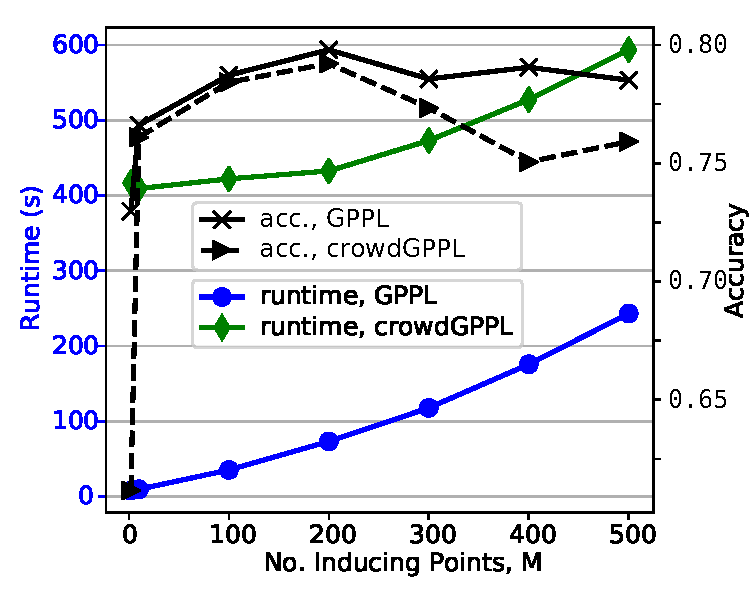
\includegraphics[clip=true,trim=12 0 12 0,width=.47\columnwidth]{num_inducing_32310_features}
}
\subfloat[Varying $N$.]{
\label{fig:Ntr}
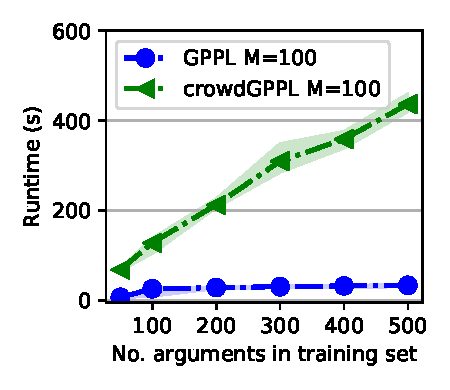
\includegraphics[clip=true,trim=11 0 11 0,width=.27\columnwidth]{num_arguments}
}
\subfloat[Varying $P$ ]{
\label{fig:Npairs}
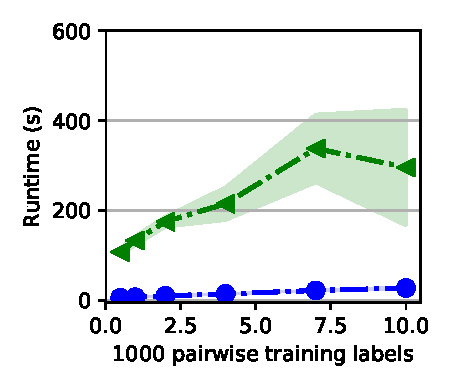
\includegraphics[clip=true,trim=49 0 10 0,width=.218\columnwidth]{num_pairs}
}
\caption{
    Wall-clock times for training+prediction of the consensus utilities 
    on UKPConvArgCrowdSample. CrowdGPPL was run with $C=5$ components. 
    Lines show means over 32 runs,
    with bands indicating one standard deviation. 
    Bands are narrow due to very little variation between folds. 
}
\end{figure}

\subsection{Posterior Variance of Item Components}
\label{sec:components}

We investigate how many latent components were actively used by 
 crowdGPPL on the \emph{UKPConvArgCrowdSample} and \emph{Sushi-A} datasets 
 using the median heuristic.
Figure \ref{fig:latent_factor_variance}
plots the posterior expectations of the inferred scales, $1/s_c$, for the latent item 
 components. 
 The plots show
that many factors have a very small variance and therefore do not contribute strongly 
to many of the model's predictions. This indicates that our Bayesian approach, in which the priors
of the latent factors have mean zero, has inferred a simpler model than the
number of latent components would permit.
\begin{figure}
\centering
\subfloat[\emph{UKPConvArgCrowdSample}]{
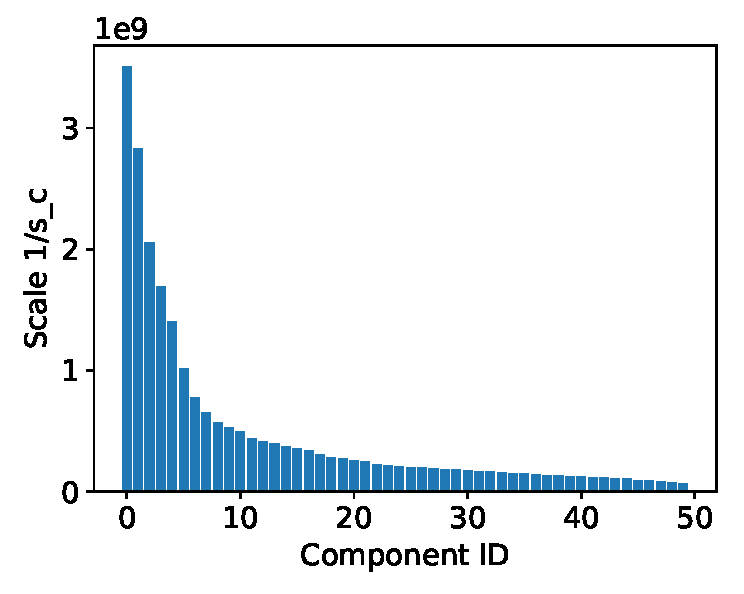
\includegraphics[trim=10 10 0 0,clip=true,width=.34\textwidth]{conv_factor_scales}
}
\subfloat[\emph{Sushi-A}]{
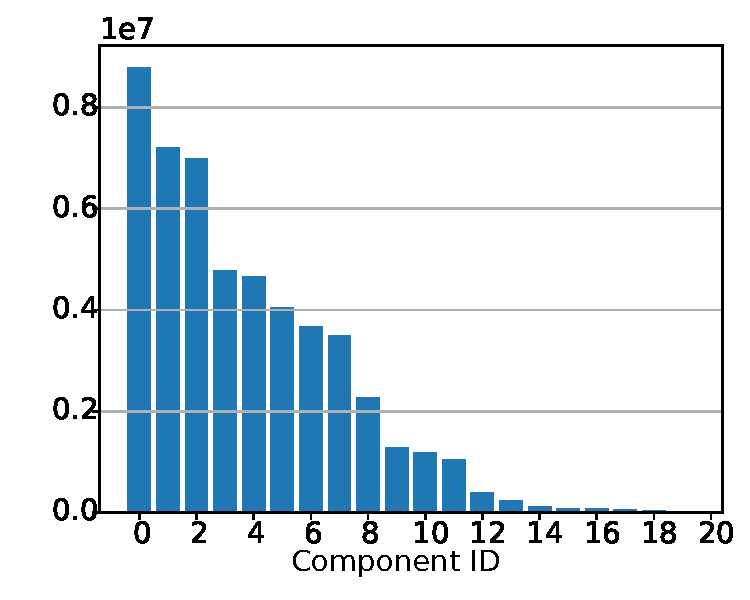
\includegraphics[trim=20 5 0 0,clip=true,width=.32\textwidth]{sushi_factor_scales}
}
\caption{
Distribution of latent component variances, $1/s_c$ in crowdGPPL, means over all runs.
}
\label{fig:latent_factor_variance}
\end{figure}
